\documentclass[12pt]{article}
\usepackage[utf8]{inputenc}

% Importing settings from setup.sty
\usepackage{setup}
\usepackage{booktabs}
\usepackage{multicol}
\usepackage{multirow}
\usepackage{glossaries}
% \makenoidxglossaries
% \newcommand{\thetahat}{\hat{\theta}}

\newacronym{emr}{EMR}{Electronic Medical Record}
\newacronym{bmi}{BMI}{Body Mass Index}


% \pagenumbering{roman}
\begin{document}

% Inserting title page
\import{./}{title}

\pagenumbering{gobble}
\tableofcontents
\listoffigures
% \listoftables



\newgeometry{
    left=25mm,
    right=25mm,
    top=25mm,
    bottom=25mm}
\pagenumbering{arabic}

\section{Exercise 1}
\section{Exercise 2}
\subsection{Question 1}
I was not familiar with the PyTorch library, so I had to perform some research in order to know how its methods/classes work.
I consulted several sources, including the following, which were useful in order to answer this question:
\begin{enumerate}
    \item \href{https://discuss.pytorch.org/t/how-sgd-works-in-pytorch/8060/2}{https://discuss.pytorch.org/t/how-sgd-works-in-pytorch/8060/2}
    \item \href{https://discuss.pytorch.org/t/performing-mini-batch-gradient-descent-or-stochastic-gradient-descent-on-a-mini-batch/21235}{https://discuss.pytorch.org/t/performing-mini-batch-gradient} \\
          \href{https://discuss.pytorch.org/t/performing-mini-batch-gradient-descent-or-stochastic-gradient-descent-on-a-mini-batch/21235}{-descent-or-stochastic-gradient-descent-on-a-mini-batch/21235}

    \item \href{https://pytorch.org/docs/stable/generated/torch.optim.SGD.html}{https://pytorch.org/docs/stable/generated/torch.optim.SGD.html}
\end{enumerate}
According to those sources, PyTorch's SGD actually computes a full-batch (vanilla) Gradient Descent, based on the data that is passed to it.
It is my understanding that in order to perform actual mini-batch (\ie where $1 < \text{batch size} < \text{number of observations}$), one simply needs to give subsets of the data a each iteration. \\
In our case, we use the full dataset in \texttt{outputs = net(inputs)}, which is why we perform full-batch GD, although we call the \texttt{optim.SGD} class.

\subsection{Question 2}
Figures \ref{fig: loss comparison 1-300}, \ref{fig: loss comparison 2-10-10} and \ref{fig: loss comparison 2-20-20} show a comparison between train and test cross entropy loss.
The leftmost diagrams have a linear scale for the vertical axis, while the rightmost diagrams have a logarithmic scale for the vertical axis.
Beware that the number of epochs varies significantly between figures.
Indeed, more pararmeters in the network implies longer training times per epoch, which in turn means that running for the same time both experiments results in different number of epochs. \\
\begin{figure}[ht]
    \centering
    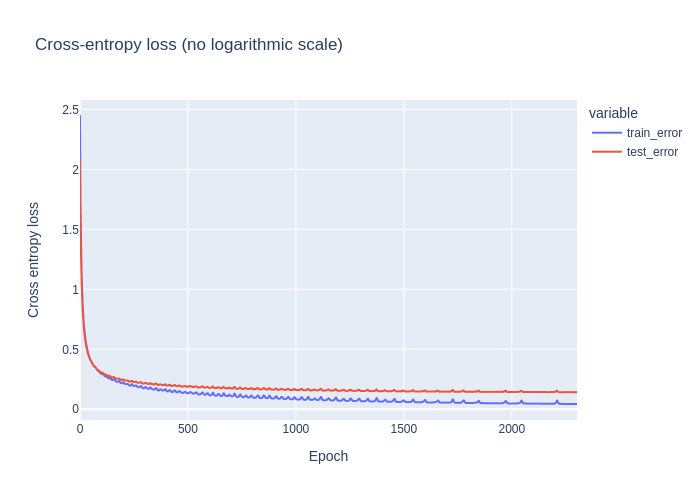
\includegraphics[width=0.49\textwidth]{images/cross-entropy-comparison-1-300.png}
    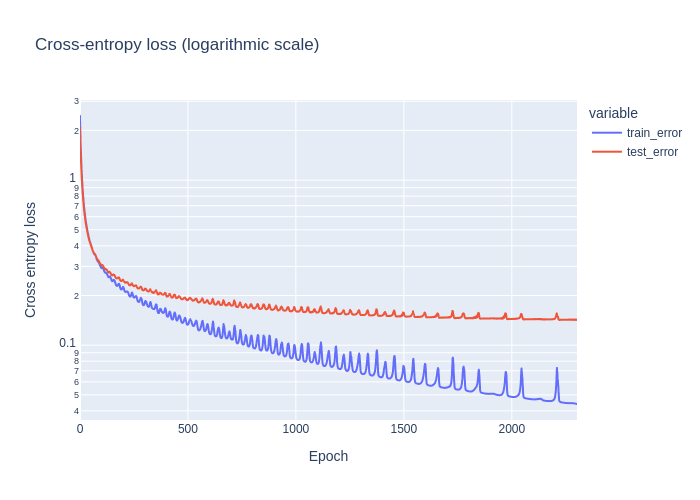
\includegraphics[width=0.49\textwidth]{images/cross-entropy-comparison-1-300-log.png}
    \caption{Cross entropy loss, train vs test ($300$ fully-connected).}
    \label{fig: loss comparison 1-300}
\end{figure}
\begin{figure}[ht]
    \centering
    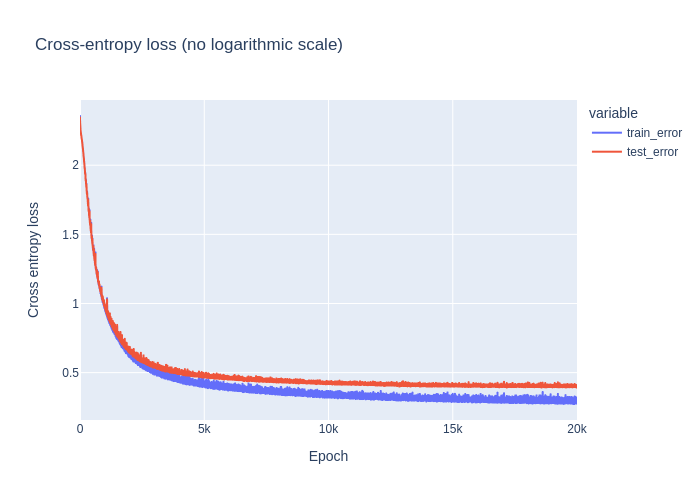
\includegraphics[width=0.49\textwidth]{images/cross-entropy-comparison-2-10-10.png}
    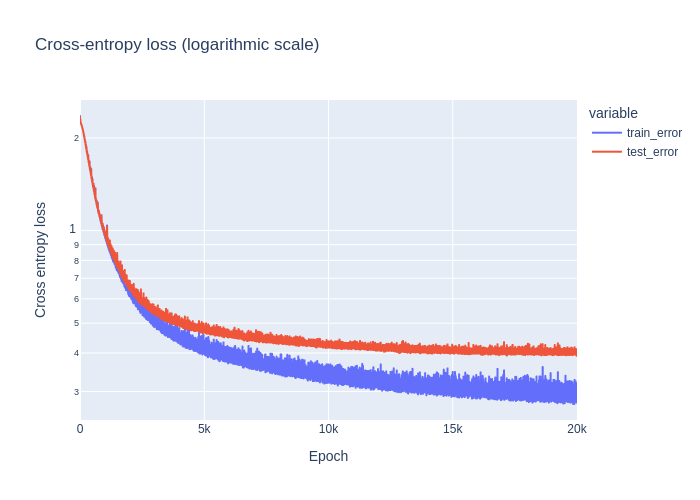
\includegraphics[width=0.49\textwidth]{images/cross-entropy-comparison-2-10-10-log.png}
    \caption{Cross entropy loss, train vs test ($10-10$ fully-connected).}
    \label{fig: loss comparison 2-10-10}
\end{figure}
\begin{figure}[ht]
    \centering
    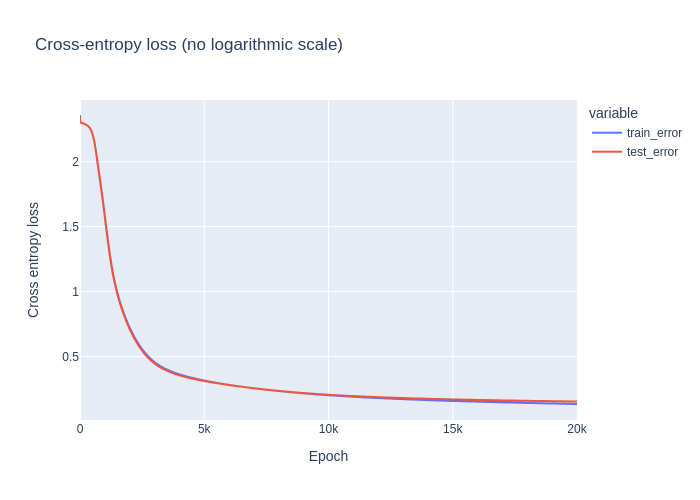
\includegraphics[width=0.49\textwidth]{images/cross-entropy-comparison-2-20-20.png}
    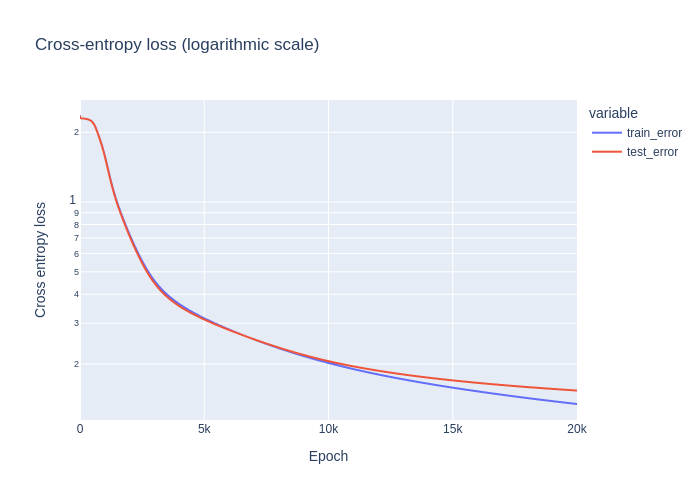
\includegraphics[width=0.49\textwidth]{images/cross-entropy-comparison-2-20-20-log.png}
    \caption{Cross entropy loss, train vs test ($20-20$ fully-connected).}
    \label{fig: loss comparison 2-20-20}
\end{figure}
We see that in both experiments the train error keeps decreasing, while the test error stays constant.
This means that our network is overfitting and there is no need to continue the experiment further.
One way to prevent wasting time training when the network isn't making actual progress is to print the loss, or even to plot the loss curves, every couple iterations.
We estimate however that the over-fitting phenomenon isn't too extreme in our case.

\subsection{Question 3}
Let $\beta: \N^{l+1} \to \N$ denote the number of parameters in a fully connected neural network. Then $\beta$ is given by:
\begin{equation}
    \beta(h_0, \ldots, h_l) := \sum_{i=1}^{l} (h_{i-1} * h_{i}) + h_i
\end{equation}
Indeed, the multiplication term ``$h_{i-1} * h_{i}$'' accounts for the weights by counting the connections from a layer to the next.
The last term ``$h_i$'' is responsible for counting the biases on each of the hidden layers, as well as the output layer. \\
We compute $\beta$ for each of our network architectures above, with $h_0 = 28 * 28 = 784$ in all cases, since this is the size of the input:
\begin{align*}
    \beta(784, 10, 10, 10)
     & = (784 * 10 + 10) + (10 * 10 + 10) + (10 * 10 + 10) \\
     & = 7850 + 110 + 110                                  \\
     & = 8070                                              \\
\end{align*}


\subsection{Question 4}

\subsection{Question 5}

\subsection{Question 6}

\subsection{Question 7}

\end{document}